\documentclass{article}
\usepackage[nonatbib]{nips_2016}

\usepackage[breaklinks=true,letterpaper=true,colorlinks,citecolor=black,bookmarks=false]{hyperref}

\usepackage{amsthm}
\usepackage{amsmath,amssymb}
\usepackage{enumitem}

\usepackage[sort&compress,numbers]{natbib}
\usepackage[normalem]{ulem}

% use Times
\usepackage{times}
% For figures
\usepackage{graphicx} % more modern
%\usepackage{epsfig} % less modern
%\usepackage{subfig}

\graphicspath{{../fig/}}

\usepackage{tikz}
\usepackage{tkz-tab}
\usepackage{caption}
\usepackage{subcaption}
\usetikzlibrary{shapes.geometric, arrows}
\tikzstyle{arrow} = [very thick,->,>=stealth]

\usepackage{cleveref}
\usepackage{setspace}
\usepackage{wrapfig}
%\usepackage[ruled]{algorithm}
\usepackage{algpseudocode}
\usepackage[noend,linesnumbered]{algorithm2e}

\usepackage[disable]{todonotes}

\usepackage{algpseudocode}

\usepackage{amsmath}
\usepackage{booktabs}
\usepackage{multirow}
\usepackage{titlesec}

\newcommand{\red}[1]{\textcolor{red}{#1}}


\title{Dynamic Model Construction for Efficient Classification}

\author{
    Jaejun Lee \\
    School of Computer Science\\
    University of Waterloo\\
    Waterloo, ON, N2L 3G1 \\
    \texttt{j474lee@uwaterloo.ca} \\
}

\begin{document}
\maketitle

\begin{abstract}

One of the major drawback of neural network based classifier is that retraining is inevitable when target set of classes changes. For this reason, such networks are often designed to be wide and deep to support all possible classes. As a results, they are computationally expensive and can lead to unpleasant user experience. In this work, I propose Composing algorithm which allows dynamic construction of a classifier using class-level transfer learning. Composing algorithm does not require any extra computation but found to be less accurate once trained with cross entropy loss. I realize that sigmoid with binary cross entropy loss can minimize the accuracy decrease and evaluate how different loss function changes the behaviour of constructed model. After thorough experiments on MNIST, keyword spotting, and CIFAR-100, it is found that sigmoid with binary cross entropy loss is more suitable for Composing algorithm but decrease in accuracy is inevitable as number of classes increases.

\end{abstract}

\section{Introduction}

Over the last decade, neural network has became {\it de facto} approach for numerous classification problems as it leads to high accuracy~\cite{lecun1998gradient, chen2014small, krizhevsky2009learning}. However, neural network based approaches require much larger computation and less flexible than preexisting techniques. When training neural network based classifier, a set of target class must be provided in order to obtain reliable classifier. A trained model then can be deployed and classify unseen data assuming that true class of the given data belongs to target set which the model is trained on. However, in practice, this is not always the case and there exist two extreme cases where this setup falls apart.

The first case is when a set of true class contains only few classes from target class set. In this case, the trained model is considered to be an excessive representation of the true classifier and wastes the resources as it calculates probabilities for unnecessary classes. This can be avoid when a set of true class is known prior to training, by training the model to classify only the necessary classes.

The other case is when the true class of an unseen data does not exist in the target classes. Unless the model is explicitly trained to classify such class as unknown, the model will classify the unseen data to be one of target classes and such misclassification can lead to system failure. The ideal solution for this issues is to train a model again with the new class, minimizing the chance of misclassification.

However, training a neural network is a very expensive operation. It can take days to obtain reliable classifier and this hinders the efficient management of a service. To combat this issue, most of the academic works focus on minimizing resource usages of a network while preserving the highest accuracy. However, there exist an alternative solution to this problem: constructing a model dynamically adapting to the change in target set while minimizing decrease in accuracy and increase in resource usage. There are three conditions which the optimal solution must satisfy:

\begin{enumerate}
    \item \textbf{Minimal accuracy degradation} : the difference in accuracy between constructed model and the base model should be small
    \item \textbf{Dynamic class addition and removal} : it must be easy to add and remove a class from the constructed model
    \item \textbf{Efficient classification} : the constructed model should not require more computations than the base model
\end{enumerate}

In the above criteria, base model refers to a model which is trained explicitly to classify the same set of class as the constructed model.

It is found that dynamic model construction is quite challenging as the optimal solution requires a technique which considers relationship between each of the neurons and the output value for every class. In this paper, I present Composing algorithm which obtains such information by class-level transfer learning. As Composing algorithm involves mixing up the weights obtained from distinct models, I realize the limitation of standard cross entropy loss approach and show that sigmoid with binary cross entropy loss is more suitable for Composing algorithm. This has been demonstrated with a set of experiment as well. Conducted on MNIST, keyword spotting, and CIFAR-100, it is found that accuracy degradation is inevitable as number of classes increases but can be minimized when models are trained with sigmoid and binary cross entropy loss.

\section{Related Works}

Even though the three criteria for dynamic model construction are quite related, there exist distinct set of problems aiming to achieve each criteria. The three most relevant domains are: ensemble learning, multi-task learning, and transfer learning

\subsection{Ensemble Learning}
Ensemble learning is a common technique in the field of machine learning which achieves higher accuracy by combining outputs of multiple models. The most famous techniques include voting, weighting, bagging and boosting~\cite{dietterich2000ensemble, breiman1996bagging, freund1996experiments}. Even though ensemble learning is considered to be easy to implement, ensemble learning assumes that models are independent. As a result, most ensemble learning algorithms require each model to process the input data parallel violating the efficiency requirement of the dynamic model construction problem.

\subsection{Multi-task Learning}
On the other hand, multi-task learning takes the opposite approach; combine a set of networks to share the knowledge learned from each task. The key assumption is that if tasks are related, sharing knowledge throughout training will increase the performance of each network. Techniques for multi-task learning are often classified into two depending on the type of information being shared: parameter sharing and feature sharing~\cite{ruder2017overview, Caruana1993MultitaskLA, duong2015low, lu2017fully}. Its architecture and consideration of multi-tasks can be adapted to the dynamic model construction problem. However it fails to satisfy the efficiency requirements as most solutions have extra layers to share information among tasks without any modification to each model.

\subsection{Transfer Learning}

Transfer learning is inspired by the same assumption as multi-task learning; sharing knowledge among tasks can improve the performance. However, the key difference between two problems is that transfer learning use the same model architecture for different tasks. Transfer learning involves pre-training and fine-tuning. First, a model is pre-trained on a task and learns to select important features. Then the same model is fine-tuned for a target task as trained weights are adjusted to produce the best result for the target task~\cite{yosinski2014transferable}. It is found that transfer learning is very powerful as demonstrated in a wide range of problems~\cite{raina2007self, egan2004effects, glorot2011domain}. Unlike two aforementioned domains, transfer learning does not add any computations for the fine-tuned task. However, knowledge sharing is mostly studied on task-level and limited work exists for class-level transfer learning.

\section{Composing Algorithm}

In this section, I introduce Composing algorithm which enables dynamic model construction for efficient classification. I also discuss the necessary conditions to achieve the best accuracy from Composing algorithm.

\subsection{Approach}

\begin{figure*}[t!]
  \centering
  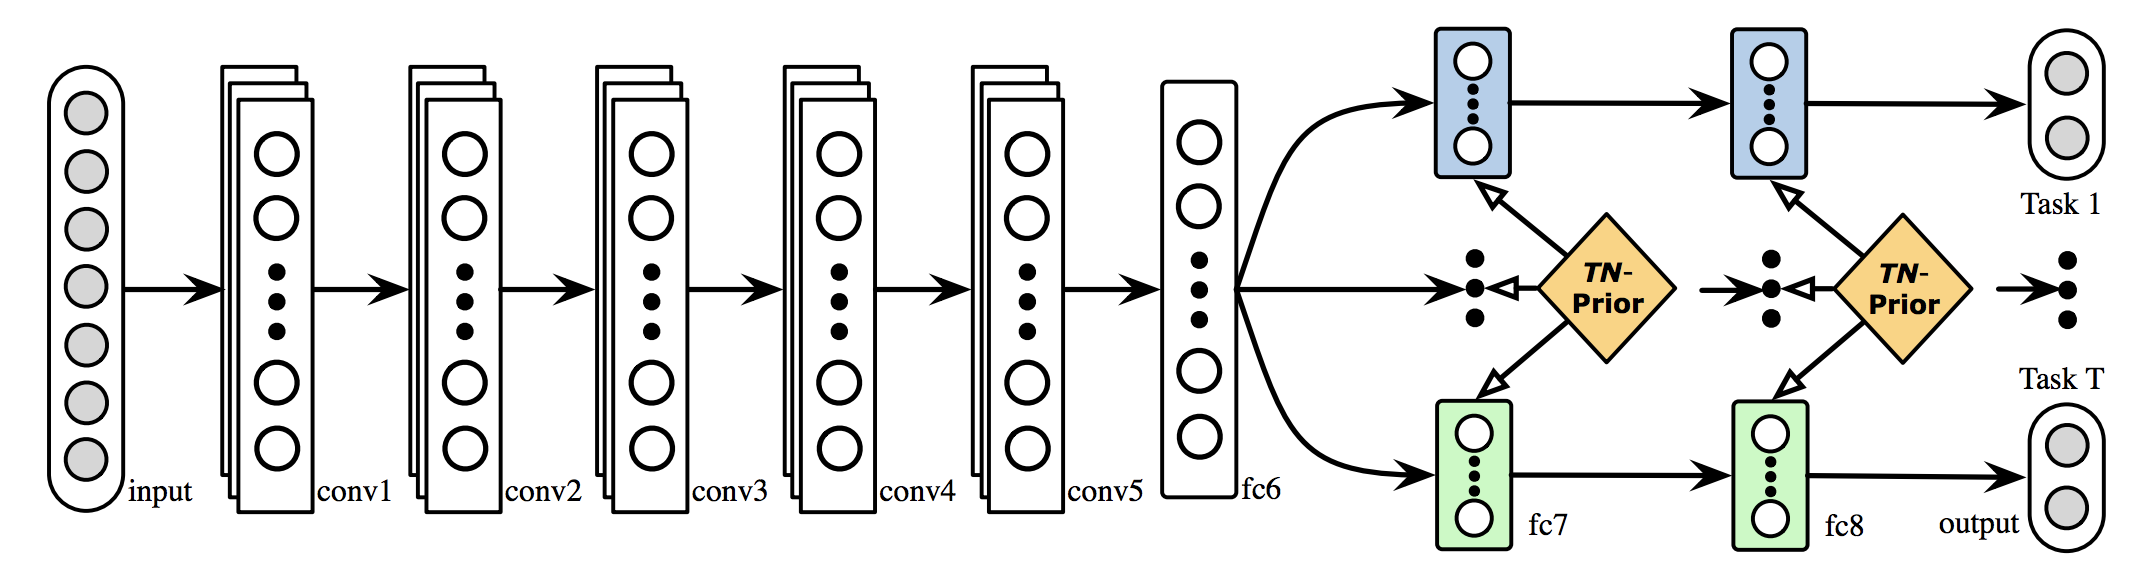
\includegraphics[scale=0.32,trim={0mm 0mm 0mm 0mm},clip]{long2017learning.png}
\end{figure*}

\begin{figure*}[t!]
	\centering
	\begin{subfigure}[b]{.65\linewidth}
		\centering
		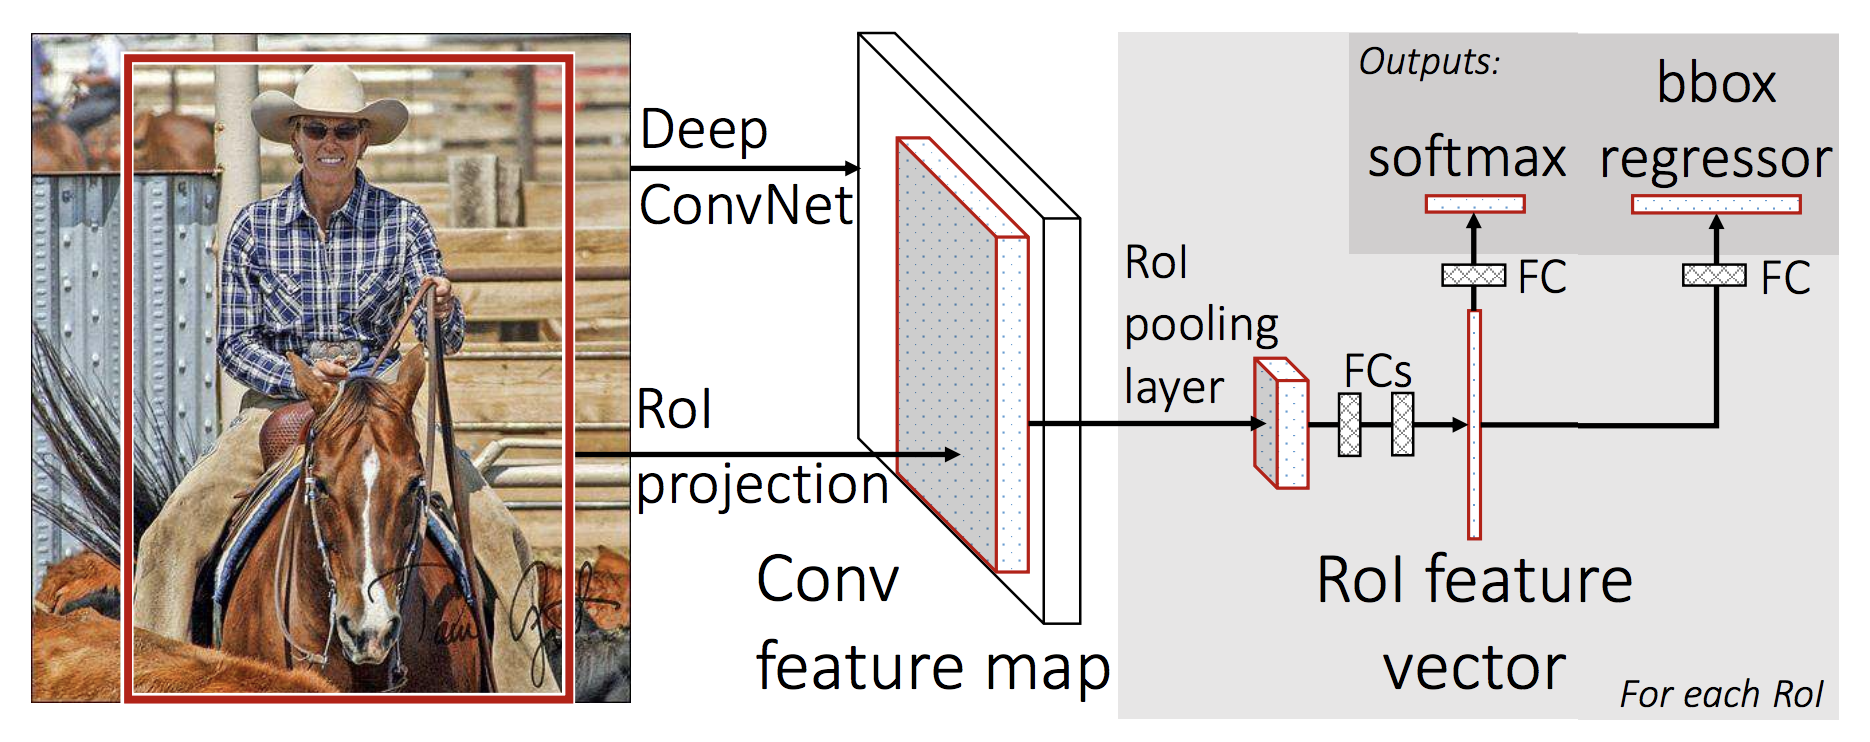
\includegraphics[scale=0.25,trim={0mm 0mm 0mm 0mm},clip]{girshick2015fast.png}
	\end{subfigure}%
	\begin{subfigure}[b]{.35\linewidth}
		\centering
		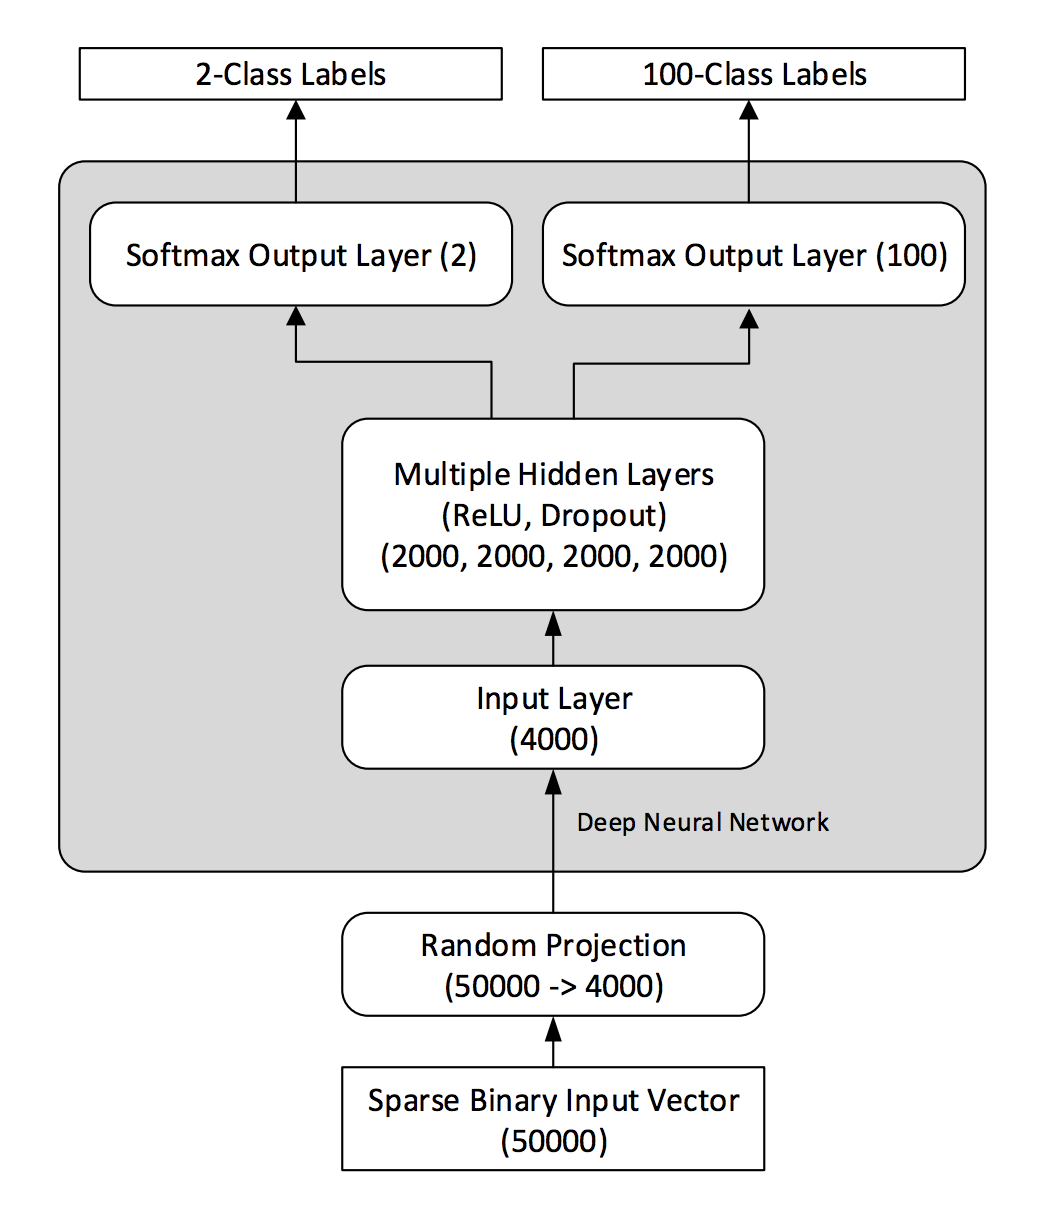
\includegraphics[scale=0.15,trim={0mm 0mm 0mm 0mm},clip]{huang2016mtnet.png}
	\end{subfigure}
	\caption{Model architectures proposed by ~\cite{long2017learning} (top), ~\cite{huang2016mtnet} (bottom right), and  ~\cite{girshick2015fast} (bottom left); Their approach for multi-task learning is to assign distinct fully-connected layer for each task.}
	\label{figure:mutli-task-learning}
\end{figure*}

One of the technique proposed for multi-task learning is to share every layer while assigning distinct fully-connected layer for each task (see Figure~\ref{figure:mutli-task-learning}). With such architecture, each task is trained independently while weights for upstream layers are shared among tasks. Once the training completes for the combined model, a task can be discarded from populating output by removing corresponding fully-connected layer. Once the trained model is left with a single fully-connected layer, it has the same architecture as the model explicitly trained to achieve the remaining task.

Recall the criteria for dynamic model construction. Once the above multi-task learning approach is applied for class-level model training, dynamic addition and removal of a class is possible and the efficiency requirement can also be satisfied. Therefore, proposed algorithm has following step:

\begin{enumerate}
    \item Pre-train a model as if it is multi-classification problem
    \item Freeze the model parameters
    \item Construct a new dataset which labels one class as positive and the others as negative.
    \item Replace the last full-connected layer for two outputs
    \item Fine-tune the last layer using the new dataset
    \item Retrieve class-specific weights (weights for positive class) of the fully-connected layer
    \item Repeat step 4 $\sim$ 7 for each class
    \item For every variation of target classes, it is possible to construct target set specific classifier by reconstructing the last layer with class-specific weights obtained from fine-tuning.
\end{enumerate}

For simplicity, this algorithm is referred as Composing algorithm, a model obtained from pre-training as pre-trained model, models constructed from step 4 $\sim$ 7 as fine-tuned models and a model constructed using this technique (obtained from the last step) as composed model.

Composing algorithm achieves dynamic addition and removal of a class by attaching and discarding corresponding fully-connected connections. With such flexibility, retraining a classifier is no longer necessary. Furthermore, Even though a class does not participate for pre-training, it is possible to construct a composed model with the class as long as it is fine-tuned using the same pre-trained model.

Again, only the weights for positive classes are used to construct a composed model. Therefore, the composed model has exactly the same number of parameters as the pre-trained model. In other words, composed model does not violate the efficiency requirements.

\section{Accuracy Preservation}

However, does Composing algorithm also guarantee the minimal accuracy degradation compared to pre-trained model? To answer this question, we need to understand how different loss functions affect the behaviour of the composed model.

\subsection{Limitations of cross entropy loss}

State of the art loss function for multi-classification is cross entropy (CE) loss, which transforms output by applying softmax and calculates negative log likelihood (NLL) as a measure of loss. Softmax and NLL loss are defined as following:

\begin{align*}
NegativeLogLikelihood(y, t) & = -\frac{1}{N}\sum_{i=1}^N \left[ t_i \cdot \log y_i\right] \\
y_i = Softmax(x_i) &= \frac{e^{x_i}}{\sum_{j}e^{x_j}} \\
\end{align*}

where $x$ is the output of the network and $t$ is the target, one hot encoded vector. The definition of the softmax can be summarized as calculating normalized logits of the network output. Therefore, $y$ has values between zero and one and they must sum up to one. Since multi-class classifier rely on the mutually exclusive assumption among the classes, CE loss is found to be the most suitable as it promotes the positive class while suppressing the negative classes.

However, such assumption can lead to unpredictable behaviour with Composing algorithm. When CE loss for Composing algorithm, the loss which used in fine-tuning gets computed with respect to the negative class. However, for a composed model, probability for each class is computed with class-specific weights which trained independently and a class with the highest probability is selected to be the final prediction.

For example, let us say there are three classes: A, B, and C. For fine-tuning, each dataset is constructed with two classes: a positive class and a negative class which represents all the other classes. For simplicity, positive weights are referred with lower case alphabets (a, b, and c) and negative weights with lower case alphabets with prime (a', b', and c'). During the fine-tuning process, loss is calculated in pairs as following: a -- a', b -- b', c -- c'. However, in the composing step, the last layer is constructed with weights a, b and c. As a results, there is no guarantee that the class with the highest output is in fact the class with the highest probability.

\subsection{Binary cross entropy with sigmoid}

Given that CE loss does not preserve the accuracy due to mutually exclusive assumption among classes, I analyze sigmoid with binary cross entropy (BCE) loss.

\begin{align*}
BinaryCrossEntropy(y, t) & = -\frac{1}{N}\sum_{i=1}^N \left[ t_i \cdot \log y_i + (1 - t_i) \cdot \log (1 - t_i) \right] \\
y_i = Sigmoid(y_i) &= \frac{1}{1 + e^{-x_i}} \\
\end{align*}

Unlike CE loss, both sigmoid and BCE loss treat each output independently. In other words, weights for each class in the fine-tuned model no longer depend on the output of the other class. This indicates that a composed model constructed using sigmoid with BCE loss provides more convincing results as accuracy decrease is smaller than what CE loss provides.

In multi-label classification, the same issue has been raised with CE loss~\cite{liu2017deep}. It is found that the independence guarantee provided by sigmoid and BCE loss is crucial for multi-label classification and enables successful training of a classifier.

\section{Experiments}

In order to understand the severity of accuracy decrease, I have implemented Composing algorithm on MNIST, Keyword Spotting, and CIFAR-100. Experiments are implemented with PyTorch and available on github\footnote{\url{https://github.com/ljj7975/composable-model-exp}}.

For each dataset, Composing algorithm is applied with three different loss functions. First, I include CE loss. Since PyTorch NLL loss implementation expects log probability, log is applied after softmax but it is found that this does not change my final conclusion. Next, I use sigmoid with BCE loss which is found to be more accurate than CE loss. Last loss function is softmax with BCE loss. This setting is known to be unstable because BCE loss assumes the independence among classes while softmax does not. In fact, I have observed the training collapse at some point. However, as I report accuracy from the best model, I found the results from this setting still valid and meaningful. This setting should allow me to understand how crucial sigmoid is for sigmoid with BCE loss as it simply replaces sigmoid with softmax.

In the following section, I report accuracy of every model created throughout Composing algorithm: pre-trained model, fine-tuned models, and composed model. Comparing accuracy of composed model against pre-trained model, it is possible to understand how each loss function affects the stability of Composing algorithm.

Furthermore, I report accuracy of every intermediary composed model as I add a class to construct a composed model. This reveals relationship between number of classes and the performance of composed model. Since fine-tuned accuracies varies a lot depending on the class each model is trained for, I repeat this step 10 times with random selection on the next class to add and report average.

\subsection{MNIST}

MNIST is a standard benchmark for classification~\cite{lecun1998gradient} which comprises images of handwritten digits. Among the wide range of model architecture proposed for this problem, \texttt{LeNet-5} is selected for this experiment~\cite{lecun2015lenet}. \texttt{LeNet-5} is constructed with two convolutional, one dropout and two fully connected layers. The original implementation of \texttt{LeNet-5} has 10 and 20 channels for the first two convolutional layers and produces accuracy of 98\% on MNIST dataset. Since accuracy is the prior measure of comparison in this experiments, such a high accuracy might lead to difficult analysis. Therefore, the network is modified to have 5 channels for both convolutional layers.

Both pre-trained model and fine-tuned models are trained using Adam optimizer with learning rate of 0.0001. Analyzed from 50 experiments, it is found that all three loss function leads to convergence in 5 epochs. Pre-training converges to average accuracy of 95\% and fine-tuning converges to 98\% (see Table \ref{table:mnist}).

Figure \ref{figure:composed_mnist} summarizes how the accuracy changes for composed model as number of classes increases. No matter which loss function is used for Composing algorithm, accuracy of composed model decreases as more classes contribute to composing step. However, models with softmax based loss show greater rate of decrease than model with sigmoid based loss. With CE loss, the composed model for all 10 classes has an accuracy of 85.86\%. This is relative decrease of 10.5\% compared to the pre-trained model. Composing algorithm with softmax with BCE loss is found to show the worst performance. The average final accuracy is 78.50\% which is 17.85\% relative decrease. As proven in the previous section, sigmoid with BCE loss introduces the least accuracy degradation and achieves accuracy of 95.29\% which is very similar to the accuracy of pre-trained model.

\subsection{Keyword Spotting}


\begin{table}[t]
    \centering
    \begin{tabular}{cccccc}
        \toprule[1pt]
        \multirow{2}{*}{\raisebox{-3\heavyrulewidth}{\bf Loss function}} &
        \multirow{2}{*}{\raisebox{-3\heavyrulewidth}{\bf Pre-trained }} &
        \textbf{Fine tuned} &
        \multirow{2}{*}{\raisebox{-3\heavyrulewidth}{ \bf Composed }} &
        \textbf{ Relative } \\
        & & avg (min $\sim$ max) & & \textbf{ decrease } \\
        \midrule
        LogSoftmax + NLL & 95.8 & 98.02 (96.29 $\sim$ 99.24) & 85.74 & 10.50 \\
        Softmax + BCE & 94.71 & 97.33 (95.08 $\sim$ 99.06) & 77.80 & 17.85 \\
        Sigmoid + BCE & 95.49 & 98.07 (96.74 $\sim$ 99.19) & 95.30 & 0.20 \\
        \bottomrule[1pt]
    \end{tabular}
    \caption{Average accuracy of base, fine-tuned, and composed model for MNIST (\%). Relative decrease is calculated using composed model with respect to pre-trained model.}
    \label{table:mnist}
\end{table}

\begin{figure}[t]
    \centering
    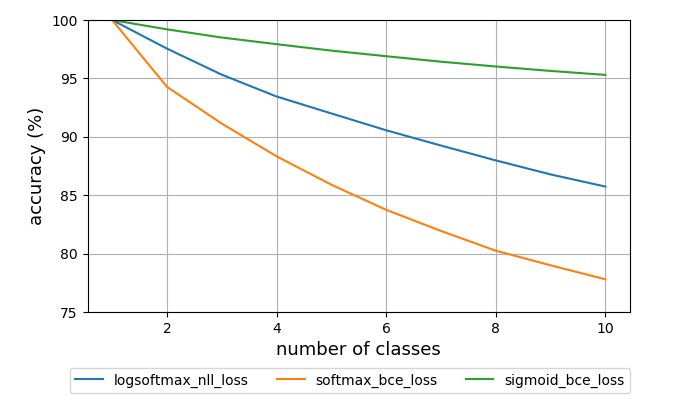
\includegraphics[scale=0.5,trim={0mm 0mm 0mm 0mm},clip]{mnist.png}
    \caption{Change in composed model accuracy with respect to number of classes for MNIST}
    \label{figure:composed_mnist}
\end{figure}


\begin{table}[t]
    \centering
    \begin{tabular}{cccccc}
        \toprule[1pt]
        \multirow{2}{*}{\raisebox{-3\heavyrulewidth}{\bf Loss function}} &
        \multirow{2}{*}{\raisebox{-3\heavyrulewidth}{\bf Pre-trained }} &
        \textbf{Fine tuned} &
        \multirow{2}{*}{\raisebox{-3\heavyrulewidth}{ \bf Composed }} &
        \textbf{ Relative } \\
        & & avg (min $\sim$ max) & & \textbf{ decrease } \\
        \midrule
        LogSoftmax + NLL & 93.09 & 95.32 (92.57 $\sim$ 97.59) & 90.13 & 3.18 \\
        Softmax + BCE & 90.94 & 91.79 (89.64 $\sim$ 94.80) & 86.78 & 4.57 \\
        Sigmoid + BCE & 89.62 & 91.31 (88.73 $\sim$ 93.91) & 88.33 & 1.44 \\
        \bottomrule[1pt]
    \end{tabular}
    \caption{Average accuracy of base, fine-tuned, and composed model for KWS (\%). Relative decrease is calculated using composed model with respect to pre-trained model.}
    \label{table:kws}
\end{table}

\begin{figure}[t]
    \centering
    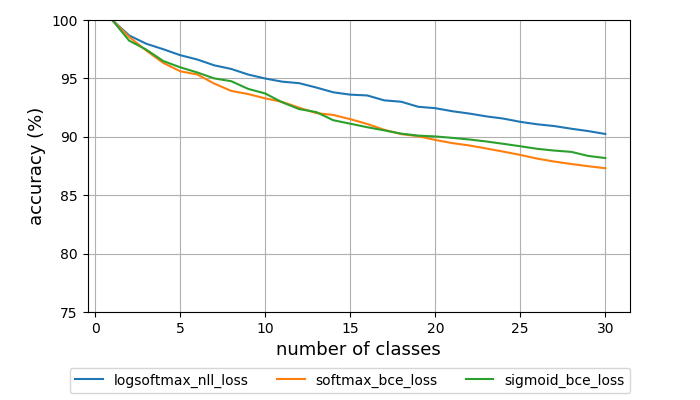
\includegraphics[scale=0.5,trim={0mm 0mm 0mm 0mm},clip]{kws.png}
    \caption{Change in composed model accuracy with respect to number of classes for KWS}
    \label{figure:composed_kws}
\end{figure}


To understand the universality of Composing algorithm, I extend this idea to keyword spotting where the input data is audio. The goal of Keyword Spotting (KWS) is to detect an audio of pre-trained keywords, such as “Hey Siri”. Since the first neural network based approach by~\cite{chen2014small}, it has became standard approach for KWS. In this experiment, I implement \texttt{res15-narrow} introduced by~\cite{tang2018deep}, which achieves accuracy of 94\% for 12 keywords on Google’s Speech Commands Dataset~\cite{speechcommandsdataset}. \texttt{res15-narrow} comprises 6 residual blocks with 19 feature maps where each residual block is composed of bias-free convolutional and batch normalization layer.

Common KWS experiments on Google’s Speech Commands Dataset involve only 12 keywords. However, since I am interested in evaluating stability of Composing algorithm with larger number of classes, all 30 keywords are used for this experiment. Following the standard feature extraction process for audio, I first construct Forty-dimensional Mel-Frequency Cepstrum Coefficient (MFCC) frames and stack them using 30ms windows with a 10ms shift. As the dataset consists of one-second long utterances of each word, the processed input has size of $101\times40$.

Throughout 10 experiments, stochastic gradient descent is used for both pre-training and fine-tuning. Training starts with learning rate of 0.1 and achieves higher accuracy as it decreases the learning rate to 0.001 by factor of ten. Base models are trained for 30 epochs with learning rate decrease at 10 and 20th epochs and fine-tuned models are trained for 10 epochs with decrease at 4 and 7th epochs.

Unlike MNIST, it is found that all three loss functions lead to reasonably good accuracy even with the composed models. First, CE loss achieves the best accuracy with \texttt{res15-narrow}; 93.09\% accuracy with the pre-trained model with average accuracy of 95.32\% with fine-tuned models. Softmax with BCE loss achieves 90.94\% accuracy with pre-trained model and average accuracy of 91.79\% with fine-tuned models. Sigmoid with BCE loss leads to the least accuracy of 89.62\% for pre-training and 91.31\% for fine-tuning.

However, Figure \ref{figure:composed_kws} shows that sigmoid with BCE loss is found to be the most reliable loss function with Composing algorithm as it shows the least relative decrease of 1.44\%. CE loss and softmax with BCE loss shows greater rate of relative decrease, 3.18\% and 4.57\% respectively. As shown from the experiments with MNIST, decrease in accuracy is also found with KWS as number of classes increases.

\subsection{CIFAR-100}
CIFAR is a collection of tiny coloured images from the web~\cite{krizhevsky2009learning}. There exist two kinds of CIFAR varying on number of classes: CIFAR-10 and CIFAR-100. The following experiment is constructed with CIFAR-100 which constitutes of 600 images of 100 classes.



\begin{table}[t]
    \centering
    \begin{tabular}{cccccc}
        \toprule[1pt]
        \multirow{2}{*}{\raisebox{-3\heavyrulewidth}{\bf Loss function}} &
        \multirow{2}{*}{\raisebox{-3\heavyrulewidth}{\bf Pre-trained }} &
        \textbf{Fine tuned} &
        \multirow{2}{*}{\raisebox{-3\heavyrulewidth}{ \bf Composed }} &
        \textbf{ Relative } \\
        & & avg (min $\sim$ max) & & \textbf{ decrease } \\
        \midrule
        LogSoftmax + NLL & 69.95 & 86.12 (71.00 $\sim$ 96.00) & 52.74 & 24.60 \\
        Softmax + BCE & 64.23 & 88.63 (79.50 $\sim$ 97.50) & 52.04 & 18.98 \\
        Sigmoid + BCE & 64.72 & 87.79 (77.50 $\sim$ 96.00) & 57.42 & 11.28 \\
        \bottomrule[1pt]
    \end{tabular}
    \caption{Accuracy of base, fine-tuned, and composed model for CIFAR-100 (\%). Relative decrease is calculated using composed model with respect to pre-trained model.}
    \label{table:cifar}
\end{table}

\begin{figure}[t]
    \centering
    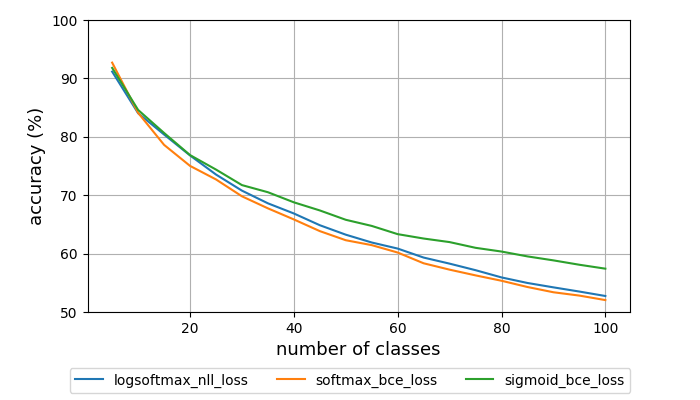
\includegraphics[scale=0.5,trim={0mm 0mm 0mm 0mm},clip]{cifar100.png}
    \caption{Accuracy of composed model for CIFAR-100 with respect to number of classes}
    \label{figure:composed_cifar}
\end{figure}


For this experiment, I have implemented \texttt{DenseNet}, a state of the art model for CIFAR dataset~\cite{huang2017densely}. Building upon a network architecture with residual connection, the feature maps of all preceding layers are used as inputs for each layer. The network has three dense blocks with transition layers between which changes the feature-map sizes by convolution and pooling. The original implementation achieves accuracy of 80\% with 300 epochs of stochastic gradient descent. Learning rate must decrease throughout the training from 0.1 to 0.001 by factor of ten.

Table \ref{table:cifar} summarizes the accuracy of models constructed throughout the experiment. As training \texttt{DenseNet} for CIFAR-100 is very expensive, only one base model has been trained for each loss functions. However, composing step is repeated 10 times, being consistent with the preceding experiments. In this experiment, the pre-training is achieved with 200 epochs and this leads to accuracy of 69.95\% for CE loss, 64.23\% for softmax with BCE loss, and 64.72\% for sigmoid with BCE loss. Fine-tuned models are trained for 100 epochs with average accuracy of 86.12\%, 88.63\%, and 87.79\% respectively.


Figure \ref{figure:composed_cifar} shows how accuracy of composed model changes as number of classes increases. It is found that CIFAR-100 introduces greater rate of decrease than MNIST and KWS. I believe this is due to the fact that CIFAR-100 involves much larger number of classes. Again, limitation of CE loss is clear as it leads to 24.60\% relative decrease with respect to the base model accuracy. Softmax with BCE loss introduces 18.98\% relative decrease while sigmoid with BCE loss shows the least decrease of 11.28\%.

\section{Discussion}

Throughout all three experiments, it is shown to have strong correlation with the number of classes. In the case of CIFAR-100, even sigmoid with BCE loss introduces relative decrease of 11.28\% which can be crucial in many cases. Therefore an algorithm which introduces the minimal accuracy decrease from the increase in number of classes would be preferred. I believe further experiments with other loss functions such as KL divergence and MSE would be helpful.

Next, when I introduce Composing algorithm, I mention fully-connected layer explicitly as the last layer. One might believe that this algorithm only works with such network as all three experiments involve network has fully-connected connections for their last layer. However, I strongly believe that this algorithm can be extended to other network as long as correct layer is selected for fine-tuning. For example, some networks apply global averaging as its last operation to minimize computation. Since global averaging does not involve any parameter, the last valid layer for fine-tuning is penultimate layer. In such networks, penultimate layer is generally convolutional layers. Therefore, as long as fine-tuning leads to reasonable accuracy and weights are loaded correctly for the new penultimate layer, the same Composing algorithm should work on these networks.

Lastly, I have shown that Composing algorithm saves computation as it does not calculate probabilities for unnecessary classes. However, as model involves more and more layers, such savings on computation may not add much benefit as this algorithm only deal with last fully-connected layer. Therefore, it is necessary to extend this idea for upstream layers and achieve greater rate of computational savings.

\section{Conclusion}

Realizing the limited flexibility of classifier, I present Composing algorithm which enables dynamic construction of a model adapting to the change in target classes. As loss function plays a key role in Composing algorithm, I study how CE loss can lead to accuracy degradation and demonstrate that sigmoid with BCE loss is more suitable. Throughout experiments conducted on MNIST, keyword spotting and CIFAR-100, I have shown feasibility of Composing algorithm. However, it is also observed that accuracy degradation is inevitable as number of classes grows.

\newpage

\nocite{*}

\bibliographystyle{unsrtnat}
\bibliography{citation}

\end{document}
